\section{Evaluation}
\label{sec:evaluation}

\subsection{Research Questions}

The evaluation is organized around three research questions. Each answer is
conditioned on a source oracle: the same workload behavior must be used for
\namei, the feature-equivalent FUSE row, and the custom/stackable
responsibility comparison.
One-off mechanism checks, source surveys, and weak baselines do not answer an
RQ by themselves.

\begin{description}
\item[RQ1] Can a narrow VFS name-resolution extension express real
state-dependent path-view policies without taking over filesystem semantics?
\item[RQ2] What is the cost of putting programmable policy on the VFS
name-resolution path compared with a feature-equivalent FUSE policy
implementation?
\item[RQ3] Does \namei provide a narrower verifier-bounded, fail-closed
ownership boundary than building a custom or stackable filesystem when the
needed policy is only name resolution?
\end{description}

\subsection{Experimental Setup}

All \namei mechanism runs execute in KVM~\cite{linux_kvm} with the modified
kernel and the real \code{cgroup/namei_ext} attach path. Make targets own the
run, attach the policy, collect raw artifacts, and fail on missing capability,
verifier failure, syscall failure, or oracle failure. Each final row records the
kernel commit, image identity, policy object, workload inputs, stdout/stderr,
dmesg, per-operation lookup/readdir events, and comparison-specific setup
observations.
Operation-weighted metrics weight each policy action by its observed frequency
in the workload trace.

Each final reported run records the kernel configuration and image identity,
filesystem configuration, run count, warmup rule, confidence-interval method,
cache protocol, compared implementation, source commit, and raw observations.

Correctness gates every number. A FUSE row is used for RQ2 only after it
implements the same policy over the same source oracle. No-hook and
lower-filesystem rows calibrate fixed hook and measurement cost. They are not
competing baselines. RQ3 executes a matched Wrapfs-derived implementation for
the Agent workspace oracle and compares responsibility and containment rather
than throughput.

\subsection{RQ1: Expressiveness And Sufficiency}

RQ1 asks whether the VFS boundary can express path-view transitions extracted
from source oracles while preserving lower-filesystem semantics. A reportable
row must pass the source oracle through the real KVM attach path and show that
\namei changed only lookup or directory visibility, while runtime orchestration,
storage state, synthetic contents, writes, and data-path behavior remain with
the source system or lower filesystem.

\begin{table}[t]
\centering
\scriptsize
\begin{tabular}{@{}L{0.18\linewidth}L{0.28\linewidth}L{0.23\linewidth}L{0.21\linewidth}@{}}
\hline
Workload & Source oracle & \namei evidence & Result evidence \\
\hline
Application file sharing (supporting)~\cite{xdg_documents_portal} & The XDG
Documents portal grant state selects one existing host document for one
application and hides it from another. & \namei selects or hides the document
by application and grant state. & Three fresh KVM boots passed 15/15 states:
3 granted views, 12 hidden views, exact logical/lower object identity, and
unchanged lower and unrelated objects. \\
Agent workspaces~\cite{agentfs_repo,swe_factory_repo,swe_factory_gym_dataset} & AgentFS-derived branch
state selects staged/base objects and hides whiteouts; a released Click task
distinguishes base from completed source. & \namei selects or hides existing
lower objects; the lower filesystem retains permissions, writes, metadata, and
file data. & The lifecycle matrix recorded 1,170 pass-bearing records with zero
failed oracles plus six metadata records in each of three runs. Three fresh
source-task boots passed 12/12 policy-backed task states and 6/6 physical
source controls: concurrent base/completed views produced 39/40 and 40/40
tests, followed by switch, rollback, and withdrawal. \\
Build action sandboxing (supporting)~\cite{bazel_sandboxing} & Two concurrent Bazel actions
use one logical input path but different declared roots; an undeclared existing
input must be absent. & \namei selects each action's declared object and hides
the undeclared name. & Three fresh KVM boots completed all six Bazel 6.5.0
actions, matched six logical/lower input objects, hid undeclared inputs, and
preserved 12 lower objects. \\
Toolchain environments (supporting)~\cite{nix_store} & Two installed
environments expose distinct interpreter and package trees; one process-group
view switches and rolls back. & \namei selects the existing environment root
without changing the logical executable path. & Three fresh KVM boots passed
18/18 physical/logical states, 24/24 Python probes, concurrent 3.10/3.12 views,
switch, rollback, and lower-object controls. \\
Kubernetes ConfigMap publication
(supporting)~\cite{kubernetes_projected_volumes,kubernetes_configmaps} &
Official \code{AtomicWriter} publication exposes V0, V1, repeated V1, and
rollback V0 payloads under one stable root. & \namei selects or hides
already-materialized leaf objects while VFS retains modes, ownership, open
descriptors, and lower objects. & Three fresh KVM boots passed 12/12 source
states, 12/12 \namei states, 6/6 direct controls, 24/24 stable-root
descriptor checks, 12/12 old-descriptor checks, and 36/36 lower-object checks. \\
\hline
\end{tabular}
\caption{RQ1 answer table. A row becomes evidence only after the source-oracle
run passes through the real KVM attach path and lower-filesystem semantics are
preserved.}
\label{tab:rq1-evidence}
\end{table}
\FloatBarrier

The required RQ1 evidence is a reviewed KVM pass/fail matrix that preserves
lookup/readdir coherence and lower-filesystem behavior for each admitted source
oracle. A workload is outside \namei's boundary if the oracle needs synthetic
contents, data-path mediation, write-conflict handling, or custom metadata
ownership in the common path.

\subsection{RQ2: Cost Versus FUSE}

RQ2 isolates the placement cost of policy by comparing \namei with a
feature-equivalent FUSE policy service under the same oracle. Non-name-resolution
lifecycle behavior is delegated identically in both rows. RQ2 does not compare
different runtimes. Instead, it compares placing the same lookup/readdir
decision inside VFS name resolution with placing it in a FUSE request path.

\begin{table}[t]
\centering
\scriptsize
\begin{tabular}{@{}L{0.2\linewidth}L{0.26\linewidth}L{0.23\linewidth}L{0.21\linewidth}@{}}
\hline
Workload & Feature-equivalent FUSE comparison & Metrics & Result evidence \\
\hline
Agent workspace lifecycle & Same 48-oracle lifecycle in \namei and a
feature-equivalent FUSE policy service. & Ten paired blocks, 20 KVM boots,
10,000 samples per mechanism. & 960/960 oracles passed. Lifecycle p50 was
5.51\,\(\mu\)s versus 62.64\,\(\mu\)s; paired FUSE/\namei ratio was
11.32\(\times\) [11.24, 11.64]. \\
FxMark cache-hot path walks & Stock, patched-unattached, attached \code{PASS},
same-filesystem \code{SELECT}, and multithreaded cached FUSE. & 50 fresh KVM
boots, 450 cells over MRPL, MRPM, and MRPH at one/two/four workers. & 450/450 cells passed.
\code{SELECT}/FUSE was 1.052--1.088\(\times\), with every paired 95\% CI above
one; complete \code{SELECT} retained 0.895--0.931 of unattached throughput. \\
Corrected FxMark directory enumeration & Same five conditions over
private-directory MRDL and shared-directory MRDM. & Ten paired blocks, 50
fresh KVM boots, and 300 cells at one/two/four workers. & 300/300 cells passed.
\code{SELECT}/FUSE was 2.20--3.66\(\times\) with CIs above one in five cells;
MRDM/4 was 1.018 [0.907, 1.135]. \\
Unused fast path & Stock versus patched-unattached cache-hot MRPL in 30 paired
blocks. & 60 fresh KVM boots and 180 cells. &
Unattached/stock was 1.0009 [0.9921, 1.0036], 1.0083 [0.9950, 1.0179], and
1.0007 [0.9918, 1.0139] at one/two/four workers. \\
\hline
\end{tabular}
\caption{RQ2 evidence table. FUSE numbers are interpreted only after the FUSE row
implements the same source policy and passes the same source oracle.}
\label{tab:rq2-evidence}
\end{table}

\begin{figure}[t]
\centering
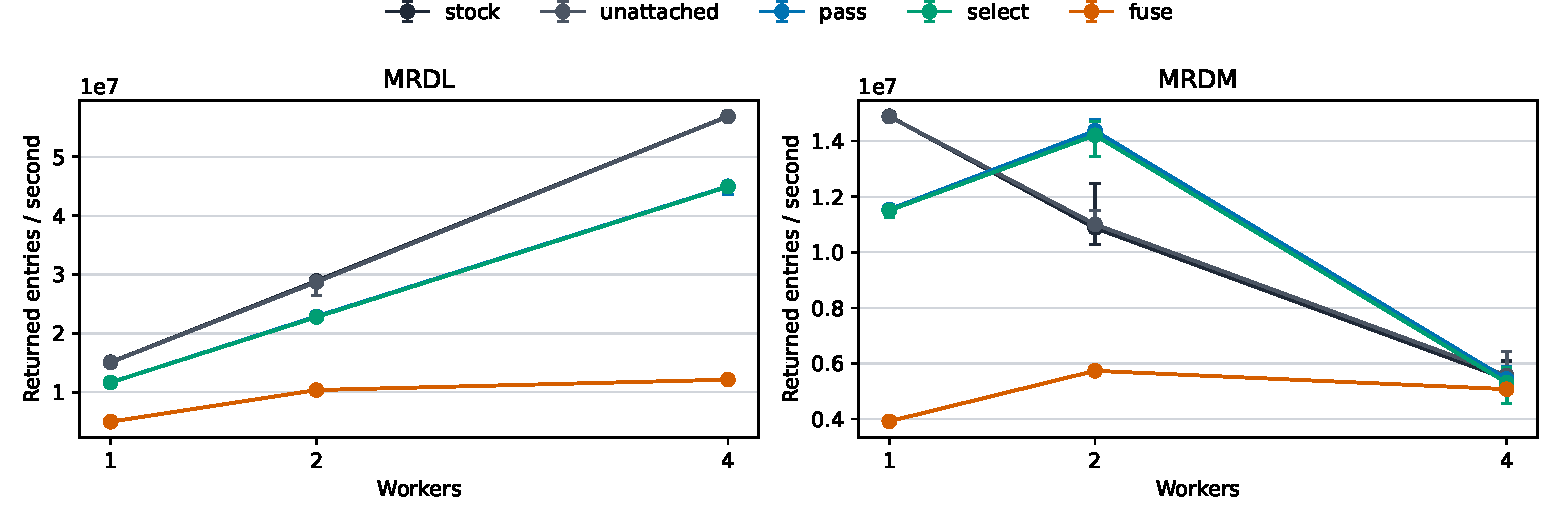
\includegraphics[width=\linewidth]{../../results/experiments/fxmark-readdir/20260729T082800Z-fxmark-readdir-formal-v1/analysis/throughput.pdf}
\caption{Corrected FxMark directory-enumeration throughput. Points are medians
over ten fresh-boot blocks; error bars are 95\% bootstrap intervals.
MRDL gives each worker a private directory; MRDM makes all workers enumerate
one shared directory.}
\label{fig:fxmark-readdir}
\end{figure}
\FloatBarrier

The Agent result is a mechanism-level lifecycle comparison, not an end-to-end
agent-task speedup. The FxMark FUSE view enabled metadata and kernel caching and
issued only 0--19 measured requests per cell; its result does not depend on one
daemon round trip per lookup. Attached \code{PASS} retained 0.901--0.934 of
unattached throughput, while \code{SELECT}/\code{PASS} was 0.981--0.999. The
separate unused-path run supports only cache-hot MRPL on this host; cold caches,
other operations, tail latency, and other machines remain open.

Figure~\ref{fig:fxmark-readdir} broadens RQ2 to the event where the BPF policy
runs for every returned directory entry. For private directories,
\code{SELECT}/FUSE is 2.200--3.663\(\times\), and \code{SELECT} scales
3.844\(\times\) from one to four workers versus 2.411\(\times\) for FUSE.
Shared-directory enumeration is 2.909\(\times\) and 2.450\(\times\) at one and
two workers. At four workers, stock, \code{SELECT}, and FUSE converge near five
million entries/s; the \code{SELECT}/FUSE interval crosses one. The frozen
overall verdict is therefore mixed: five cells support the throughput
advantage, while shared-directory contention masks it in the sixth.

\subsection{RQ3: Ownership And Containment Boundary}

RQ3 compares ownership boundaries for the same oracle-relevant behavior. The
question is not whether custom or stackable filesystems are expressive, because
they are. The question is whether the workload needs that broader boundary when
the policy effect is only name-resolution selection or visibility.

\begin{table}[t]
\centering
\scriptsize
\setlength{\tabcolsep}{3pt}
\begin{tabular}{@{}L{0.18\linewidth}L{0.20\linewidth}L{0.20\linewidth}L{0.20\linewidth}L{0.16\linewidth}@{}}
\hline
Evidence & \namei & Wrapfs-derived & Runtime/fault observation & Result \\
\hline
Agent workspace, same 37-row oracle & BPF decides lookup/readdir; ordinary
operations use the selected ext4 object. & A port of official Wrapfs registers
34 unique VFS slots across six compiled sources. & Thirteen Wrapfs method
classes executed. After \namei detach, an open descriptor completed ordinary
lower-file operations without re-entering BPF. & 37/37 oracles passed for
both mechanisms in each of three KVM boots. \\
Invalid policy/output matrix & Verifier rejects invalid programs; kernel
returns declared errors for malformed or unsupported decisions. & Validation
and failures remain kernel-module filesystem responsibilities. & Two verifier
cases produced exact rejection logs; 19 independent runtime faults each
preserved exact lower-object evidence. & 21/21 cells passed in each of three
boots. \\
\hline
\end{tabular}
\caption{RQ3 boundary table. The comparison is responsibility and containment for
the same oracle-relevant behavior, not a claim that custom filesystems are less
expressive.}
\label{tab:rq3-evidence}
\end{table}
\FloatBarrier

For this existing-object workspace view, RQ3 is supported: \namei confines
workload policy execution to lookup and directory iteration, while the matched
stackable implementation owns and executes superblock, lookup, directory,
inode, and file methods. This is a workload-specific ownership and containment
result. It is not proof of complete-system security, nor a claim that custom
filesystems are unnecessary when an oracle requires synthetic contents,
copy-up, conflict resolution, distributed metadata, or data-path mediation.

\subsection{Evaluation Scope}

The completed evidence includes five reviewed formal RQ1 workflows, an Agent
lifecycle RQ2 comparison, cache-hot FxMark
active and unused-path results, a formal corrected-FxMark directory-enumeration
matrix, and one matched Agent-workspace RQ3 boundary experiment. A historical
ccache compile matrix is
supporting macro evidence: its hot-cache run observed FUSE/\namei 2.18\(\times\)
and native/\namei 0.945\(\times\), but it lacks independent-run uncertainty and
release-scale miss/stale/corrupt cells. It is not a headline workload because
ccache already implements cache lookup and validation in userspace.

Full service validation/reload, checkpoint/restore, and HPC staging remain
portfolio extensions rather than completed evidence. The Kubernetes result
covers already-materialized payload selection and visibility, not ConfigMap
retrieval, symlink/inotify behavior, or application reload. Cache-cold lookup,
broader metadata operations, tail latency, and a second
source-derived RQ3 row remain open. Materialized namespaces, eBPF LSM, and
native source mechanisms remain related work unless a fixed source oracle makes
one a direct comparison.
